\documentclass[11pt,a4paper,notitlepage]{article}

    \usepackage[margin=1in]{geometry}
    \usepackage{algorithm}
    \usepackage{algpseudocode}
    \usepackage{graphicx}
    \usepackage{subcaption}
    \usepackage{mwe}
    \usepackage{amsmath}
    \usepackage{float}
    \usepackage{multicol}

    \title{CCS - Network Analysis Assignment}
    \author{Fatema Alkhanaizi}
    \date{\today}

\begin{document}

\graphicspath{ {../distributions/q2/} {../distributions/q1/} {../distributions/q3/} }

\maketitle

\noindent
Clearly document what you have done. For each question you should report on what you did and include, as needed, illustrative plots.

\section*{Question 1}
\subsection*{Ring Group Graph implementation}
\textbf{networkx} python3 package was used to create the graph and to check that the graph instances used for the degree distribution are fully connected (all unconnected graphs were skipped). It was also used to calculate the diameter of the graph.

\subsection*{Ring Group Graph Degree Distribution when $p + q = 0.5$, $p > q$}
\begin{itemize}
    \item Investigate the degree distribution of Ring Group Graphs for p + q = 0.5, p > q. 
    \item Decide which values of m, k, p and q to investigate. 
    \item You should report on how the structure changes as p and q vary and whether the same effects are found for different values of m and k.
    \item Use plots to illustrate your observations.
\end{itemize}
\noindent
The degree distrbution was normalized and averaged over 25 instances of the ring group graph. The following figures are for the case when $p + q = 0.5$, $p > q$:
\begin{figure}[H] 
    \centering
    \begin{minipage}{0.49\textwidth}
        \centering
        \includegraphics[width=1\textwidth]{{50-20-0.01}.png}
        \subcaption{m = 50, k = 20}
        \label{pq0.5:m50k20}
    \end{minipage}
    \begin{minipage}{0.49\textwidth}
        \centering
        \includegraphics[width=1\textwidth]{{20-50-0.01}.png}
        \subcaption{m = 20, k = 50}
        \label{pq0.5:m20k50}
    \end{minipage}
    \caption{Ring Group Graph when $p + q = 0.5$, $p > q$}
    \label{rgg:pq0.5}
\end{figure}
\noindent
By the Ring Group graph definition each vertex can be linked to 3 groups (two adjacent groups and its own group) and since each group has k members there is $p \times (3k-1)$ edges the verrex can be conneced to on average with this condition (the subtracted 1 is the vertex itself - no self edges allowed). So, the average for the remaining edges is $q \times k \times (m-3)$ (the vertices connected with p substracted from all the vertices). So, the degree distribution figures can be explained by these equation:
\begin{equation*} \label{rgg:vad}
    \mu_{degree} = p \times (3k - 1) + q \times k \times (m-3) 
\end{equation*} 
 The general shaped of the degree distribution for a Ring Group Graph is a bell shaped. A vertex average degree is heavly infllued by the value of k which is evident in figure-\ref{pq0.5:m20k50} and figure-\ref{pq0.5:m50k20}; for the same number of nodes, p and q values, the distribution in figure-\ref{pq0.5:m20k50} is shifted toward greater degree distribution than in figure-\ref{pq0.5:m50k20}.\\
 The following plots can be considered special cases which can be extrapolated from equation-\ref{rgg:vad}:
 \begin{figure}[H] 
    \centering
    \begin{minipage}{0.49\textwidth}
        \centering
        \includegraphics[width=1\textwidth]{{6-100-0.01}.png}
        \subcaption{m = 6, k = 100}
        \label{pq0.5:m6k100}
    \end{minipage}
    \begin{minipage}{0.49\textwidth}
        \centering
        \includegraphics[width=1\textwidth]{{4-100-0.1}.png}
        \subcaption{m = 4, k = 100}
        \label{pq0.5:m4k100}
    \end{minipage}
    \caption{Special cases for Ring Group Graph when $p + q = 0.5$, $p > q$}
    \label{srgg:pq0.5}
\end{figure}
\noindent
For figure-\ref{pq0.5:m6k100}, by equation-\ref{rgg:vad} when m = 6 we get:
$$ \mu_{degree} = p \times (3k - 1) + q \times 3k $$
so for this distribution regardless of the value of k combinations of p and q where $p + q = 0.5$ and $p > q$ will result in almost the same average degree across all combinations; hence the overlapped distributions in figure-\ref{pq0.5:m6k100}. 

% ToDo talk about figures 1c and 1d.


\subsection*{Diameter of Ring Group Graph and $p$ (for a fixed $q$, $p > q$)}
\begin{itemize}
    \item Investigate the relationship between the diameter of Ring Group Graphs and p (for fixed q, p > q). 
\end{itemize}
The diameter was caluculated over 20 instances of the ring group graph and run against multiple fixed q values and tested against two m and k values (20 and 50):
\begin{figure}[H]
    \centering
    \begin{minipage}{0.49\textwidth}
        \centering
        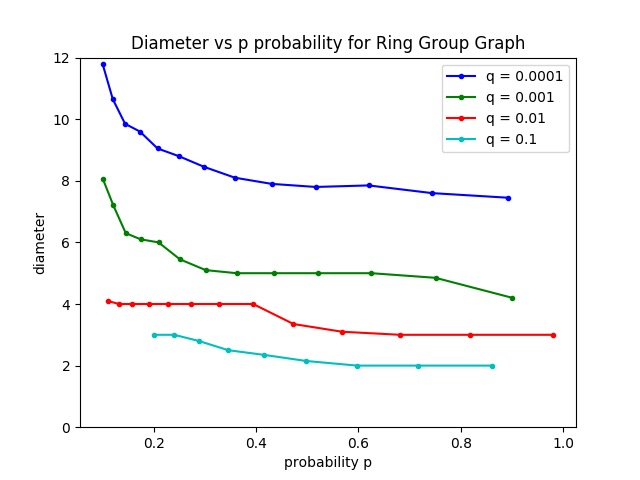
\includegraphics[width=1\textwidth]{{diameter/50-20}.png}
        \subcaption{m = 50, k = 20}
        \label{dia:m50k20}
    \end{minipage}
    \begin{minipage}{0.49\textwidth}
        \centering
        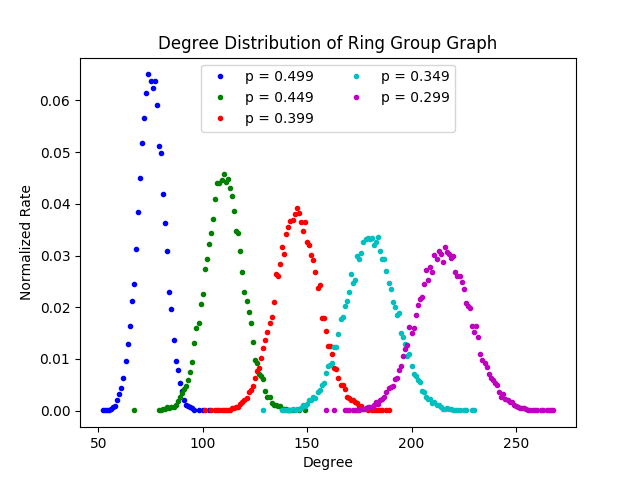
\includegraphics[width=1\textwidth]{{diameter/20-50}.png}
        \subcaption{m = 20, k = 50}
        \label{dia:m20k50}
    \end{minipage}
    \caption{Diameter for Ring Group Graph when $p > q$ ($q$ is fixed)}
    \label{rgg:dia}
\end{figure}
\noindent
The picked values for m and k provided a good contrast on how the diameter is affected when m is greater than k and vice versa. As shown in figure-\ref{rgg:dia}, as p increases the diameter decreases and at some point it becomes constant. For various q values the diamter had a similar behaviour, the value of the diameter was generally higher as q decreased which is expected as the probability q essentially creates shortcuts between the groups and without those shortcuts the diameter depends on the value of m and p. 

\begin{figure}[H]
    \centering
    \begin{minipage}{0.49\textwidth}
        \centering
        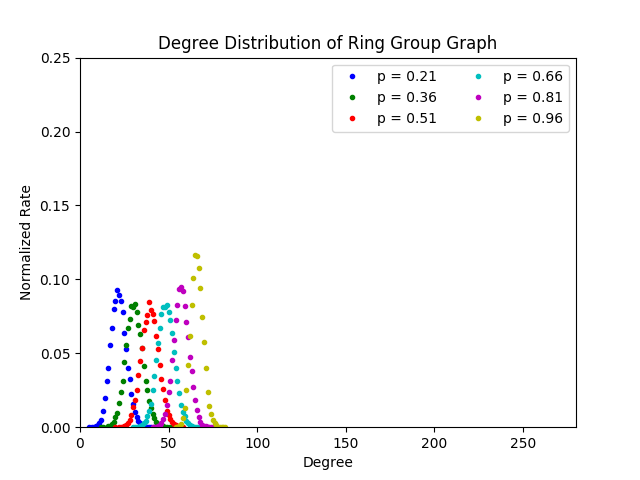
\includegraphics[width=1\textwidth]{{prob-p/50-20-0.01}.png}
        \subcaption{m = 50, k = 20, q = 0.01}
        \label{dd:m50k20}
    \end{minipage}
    \begin{minipage}{0.49\textwidth}
        \centering
        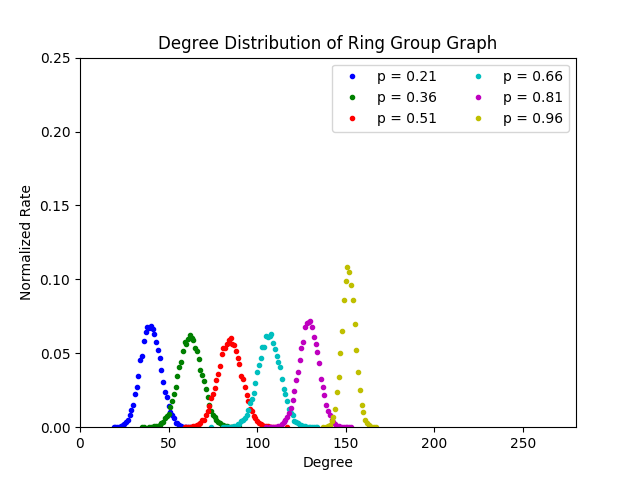
\includegraphics[width=1\textwidth]{{prob-p/20-50-0.01}.png}
        \subcaption{m = 20, k = 50, q = 0.01}
        \label{dd:m20k50}
    \end{minipage}
    \begin{minipage}{0.49\textwidth}
        \centering
        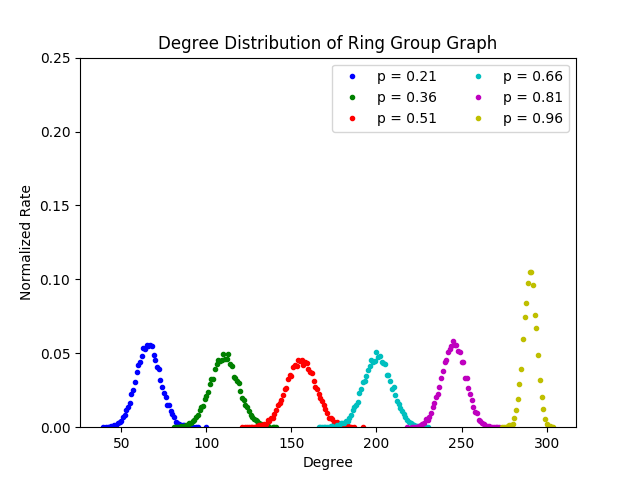
\includegraphics[width=1\textwidth]{{prob-p/6-100-0.01}.png}
        \subcaption{m = 6, k = 100, q = 0.01}
        \label{dd:m6k100}
    \end{minipage}
    \caption{Ring Group Graph when $p > q$ ($q$ is fixed)}
    \label{rgg:dd}
\end{figure}
\section*{Question 2}
\subsection*{Distribution of Vertex Brilliance}
\subsubsection*{Calculating Vertex Brilliance}
\begin{itemize}
    \item Construct the undirected graph defined in coauthorship.txt. Ignore edge weights.
    \item For the graph from coauthorship.txt, investigate the distribution of vertex brilliance. 
    \item For each of the following types of graph
    \begin{itemize}
    \item PA Graphs
    \item Ring Group Graphs 
    \end{itemize}
    create examples with approximately the same number of vertices and edges as the graph from coauthorship.txt and investigate the distribution of vertex brilliance. Comment on what you find.
\end{itemize}
The vertex brilliance was caluculated based on a similar approach to calculate the diameter by using breadth-first search but by only doing breadth-first search at debth of 2; by checking the neighbours of the vertex's neighbours. The algorithm simplified:
\begin{enumerate}
    \item create an empty dictionary; this dictionary will hold the weight vertices for the k-star of the current vertex 
    \item populate the dictionary with v's neighbours and give each vertex in the dictionary a weight of 0 to begin with < this weight will be used to determine which vertex to exclude to get the maximum k-star, the weight corresponds to how many v's neighbours the vertex is connected to
    \item repeat until maximum k-star is found
    \begin{itemize}
        \item for each vertex in the k-star dictionary go through its neighbours. If one of the vertex neighbour is a key in the k-star dictionary substract 1 from the weight of the vertex (I gave it negative value as just a notion that this is undesired vertex thus a negative affect but it can be calculated with the same manner by adding 1 but then the rest of the code will be modified so it get the maximum value from the k-star values instead of the minimum)
        \item find the minimum weight (value) of the k-star dictionary 
        \item if the minimum value is 0 then stop as this indicates that non of the vertices in the dictionary are adjacent thus it is the maximum k-star set of vertices (ther can be more than one set but we only care about the length so the actual vertices of the maximum set don't have any actual value for us in this case) so stop the loop
        \item else find the vertex with the minumum weight and remove it from the dictionary (this vertex is the most influential as it connects to the most number of vertices and by removing it the rest of vertices will be less adjacent, only the first found vertix will be removed) and reset all the other vertices values to 0 
    \end{itemize}
    \item return the length of the dictionary 
\end{enumerate}
This is essentially an algorithm to get the maximum independent set of sub-graph that only contains v and it's neighbours. I opted to using my own algorithm instead of using networkx's implementation. 
\subsubsection*{Creating Vertex Brilliance Distribution}
For each generated graphs (PA graph and Ring Group graph), the vertex brilliance distribution was averaged and normalized over 100 instances. The distribution was created following the same code as the degree distribution.

\subsection*{Vertex Brilliance Results}
\subsubsection*{Co-authorship Graph}
The co-authorship graph was loaded by following code provided in the lectures; it was just basic file-reading and making sure that the edges were undirected. The following figures are the degree distribution (in blue) and the vertex brilliance distribution (in red) of the graph:
\begin{figure}[H]
    \centering
    \begin{minipage}{0.49\textwidth}
        \centering
        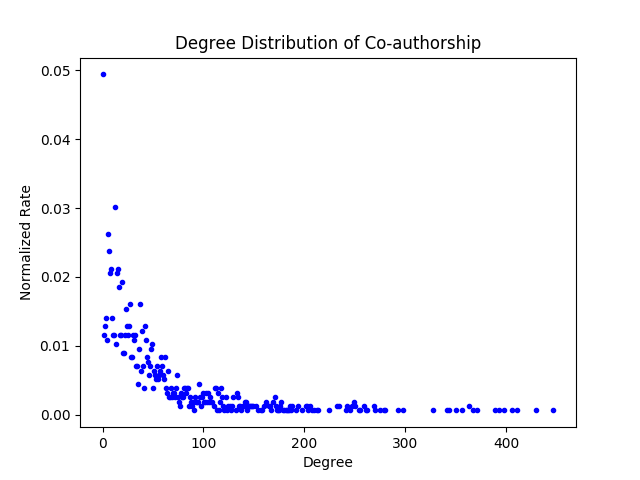
\includegraphics[width=1\textwidth]{coauthorship-vertex-degree.png}
    \end{minipage}
    \begin{minipage}{0.49\textwidth}
        \centering
        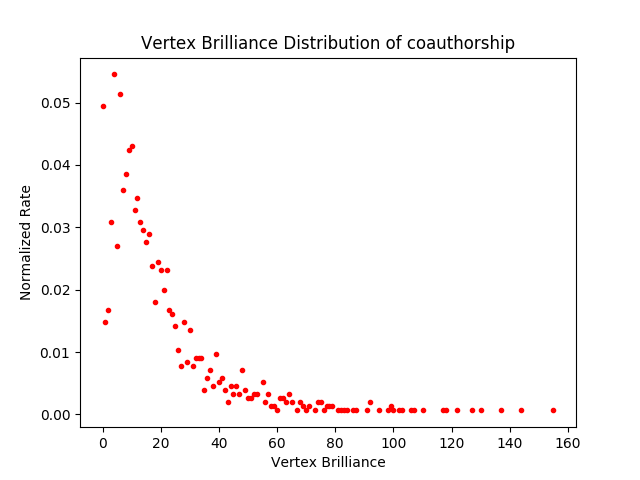
\includegraphics[width=1\textwidth]{coauthorship-vertex-brilliance.png}
    \end{minipage} \hfill
    \caption{Loaded Co-authorship Graph including vertices with no edges}
\end{figure}
The general shape of both graphs is skewed to the right.

\subsubsection*{PA Graph}
As the implementation of the PA Graph that we used in the lectures was directed, I modified networkx implementation and matched it to the PA Graph specifications provided in lecture:
\begin{itemize}
    \item I made the first 1 to m vertices fully connected and repeated each vertex m times in a list for selecting the new edges for the remaining vertices
    \item For the remaining m + 1 to n vertices, I randomly picked a vertex from the previous list m times (created an edge). For each iteration until n is reached, I added the new vertex m times in the selection list along with its neighbours.
\end{itemize} 
\begin{figure}[H]
    \centering
    \begin{minipage}{0.49\textwidth}
        \centering
        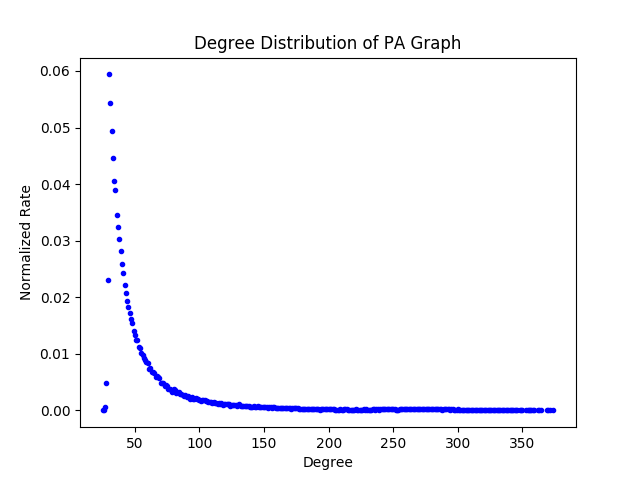
\includegraphics[width=1\textwidth]{pa_graph-1559-30-degree.png}
    \end{minipage}
    \begin{minipage}{0.49\textwidth}
        \centering
        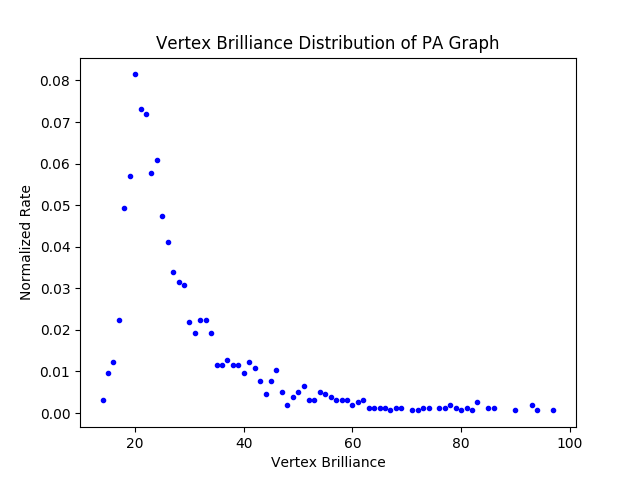
\includegraphics[width=1\textwidth]{pa_graph-1559-30-brilliance.png}
    \end{minipage} \hfill
    \caption{PA Graph parameters: m = 1559, m = 30}
\end{figure}
Both distributions has been averaged over 100 instances of the PA graph. The resulted graphs for both degree and vertex brilliance distributions are skewed to the right. The co-authorship graph strongly resembles the PA graph based on the distributions. 

\subsubsection*{Ring Group Graph}
To get approximately the same number of edges and nodes as the co-authorship graph, the following parameters were used: m = 60, k = 26, p = 0.22, q = 0.03; there are other possible parameters but their distributions are similar to the distributions with the paramaters used here (in terms of shape). 
\begin{figure}[H]
    \centering
    \begin{minipage}{0.49\textwidth}
        \centering
        \includegraphics[width=1\textwidth]{{ring_group_graph-60-26-0.22-0.03-degree}.png}
    \end{minipage}
    \begin{minipage}{0.49\textwidth}
        \centering
        \includegraphics[width=1\textwidth]{{ring_group_graph-60-26-0.22-0.03-brilliance}.png}
    \end{minipage} \hfill
    \caption{Ring Group Graph parameters: m = 60, k = 26, p = 0.22, q = 0.03}
\end{figure}
\begin{figure}[H]
    \centering
    \begin{minipage}{0.49\textwidth}
        \centering
        \includegraphics[width=1\textwidth]{{ring_group_graph-120-13-0.26-0.04-degree}.png}
    \end{minipage}
    \begin{minipage}{0.49\textwidth}
        \centering
        \includegraphics[width=1\textwidth]{{ring_group_graph-120-13-0.26-0.04-brilliance}.png}
    \end{minipage} \hfill
    \caption{Ring Group Graph parameters: m = 120, k = 13, p = 0.26, q = 0.04}
\end{figure}
Both distributions are bell shaped (binomial distribution).
\\ \\
Based on the previous graphs, it can be concluded that the vertex distribution has the same shape as the degree distribution and the co-authorship graph closely resembles the PA graph. 




\section*{Question 3}
\subsection*{Search Random Graph}
\subsubsection*{Search Algorithm}
The search in a Random Graph was implemented as follow:
\begin{itemize}
    \item Inputs:
    \begin{itemize}
        \item The graph
        \item The graph parameters - (n, p)
        \item The start vertex id - (numerical id)
        \item The target vertex id - (numerical id)
    \end{itemize}
    \item Initialize a variable for search time and set it to 0
    \item Calculate the average number of neighbours based on the number of nodes and p
    \item check if p is greater than 0.5, if it is then set p to 1 - p
    \item start an infinite loop until the target vertex is found:
    \begin{itemize}
        \item shuffle the current vertex's neighbours list (at the beginning it is the start vertex)
        \item check if the number of neighbours is more than average if so then set the number of iterations up until the average
        \item Iterate over the neighbours' list:
        \begin{itemize}
            \item increment the search time by 1 for every iteration that happens
            \item if the neighbour's id matches the target's id then stop, break out of the loop and return the search time
            \item else move to the neighbour with a probability p (the probability of the random graph)
        \end{itemize}
        \item if no moves were made move to the last queried neighbour
    \end{itemize}
\end{itemize}
The algorithm above made use of the general knowledge of the graph i.e. total number of nodes (n) and the probability (p) that an edge exists between each pair of nodes in addition to the local knowledge i.e. vertex id and number of its neighbours to better find the target vertex (t). Every vertex had the same probability to be connected to t, hence the condition to move to a node based on the probability p. Either going until the average number of neighbours or going until all the neighbours did not result in a much better search time. This is evident from the search time distribution in figure-\ref{rg:n1} and figure-\ref{rg:n2} in the next section; going only until the average number of neighbours did not improve the search time by any significant margin even for bigger values of n. Still in the above algorithm the number of iterations is maxed at the average number of neighbours. By reseting p to a lower probability when p is more than 0.5, made it less likely to move to another vertex to find the target vertex as the high probability indicates that it is very likely that the target vertex is connected to the current vertex. Another note regarding the algorithm, as the neighbours were shuffled with every move, moving to the last neighbour every time no moves happened will be random in itself as well so a different vertex will be moved to in every iteration; of course based on the probability and how random the outcome of the shuffling.

\subsubsection*{Search Time Distribution}
The search time distribution was created by searching 30,000 random pairs of vertices normalized and averaged over 10 random graph instances. To insure that the graph instance was connected, networkx package was used for both creating the graph using networkx graph structure and then checking if it's connected (all nodes have an edge between them). The plots below were created to investigate the search time distribution for a random graph and how it was affected by the total number of nodes (n) and probability p:
\begin{figure}[H]
    \centering
    \begin{minipage}{0.48\textwidth}
        \centering
        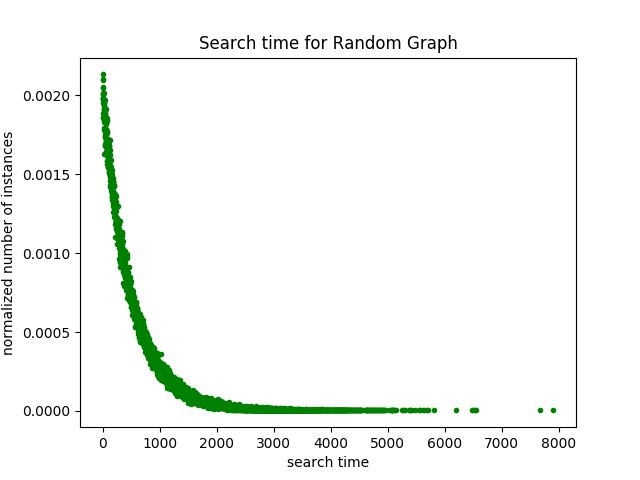
\includegraphics[width=1\textwidth]{{search-time/random_graph-500-0.1-search_time_v2-avg}.png}
        \subcaption{Normalized search time distribution}
        \label{rg:501n}
    \end{minipage}\hfill
    \begin{minipage}{0.48\textwidth}
        \centering
        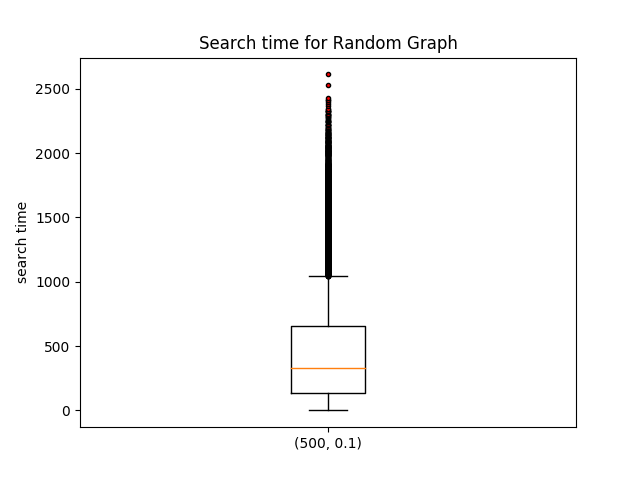
\includegraphics[width=1\textwidth]{{box/box-random_graph-500-0.1-search_time_v2-avg}.png}
        \subcaption{Box-plot respresentation of the search time distribution}
        \label{rg:501b}
    \end{minipage} \hfill
    \caption{Search Time Distribution for Random Graph when n = 500 and p = 0.1}
    \label{rg:501}
\end{figure}
\noindent
Figure-\ref{rg:501n} is an example of a search distribution for a random graph when n is 500 and p is 0.1. The box-plot will be used to represent the distribution as it is much simpler to interupt like figure-\ref{rg:501b}; some of the outlier values might not be included, those outliers have a low number of occurance so they were discarded in the box-plot and only the main distribution was included. In this case, the distrbution was skewed to the right with a lot of outlier values. More than $50\%$ of the instances had a search time that was less than 500. The median search time was roughly around 300 for this graph instance. 
\begin{figure}[H]
    \centering
    \begin{minipage}{0.48\textwidth}
        \centering
        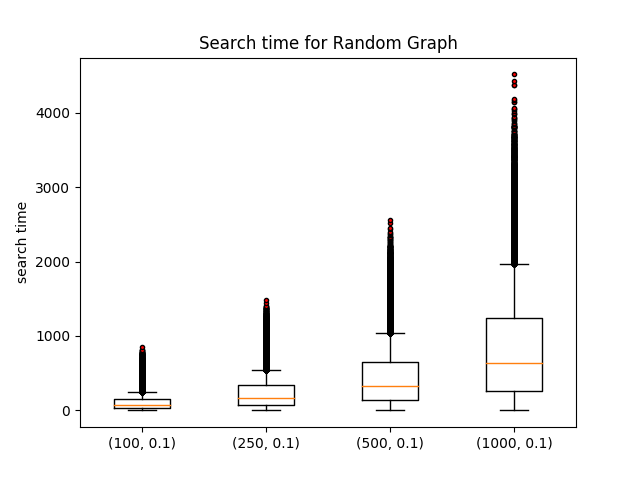
\includegraphics[width=1\textwidth]{{box/box-random_graph-n-search_time_v1-avg}.png}
        \subcaption{Only iterate until average number of neighbours}
        \label{rg:n1}
    \end{minipage}\hfill
    \begin{minipage}{0.48\textwidth}
        \centering
        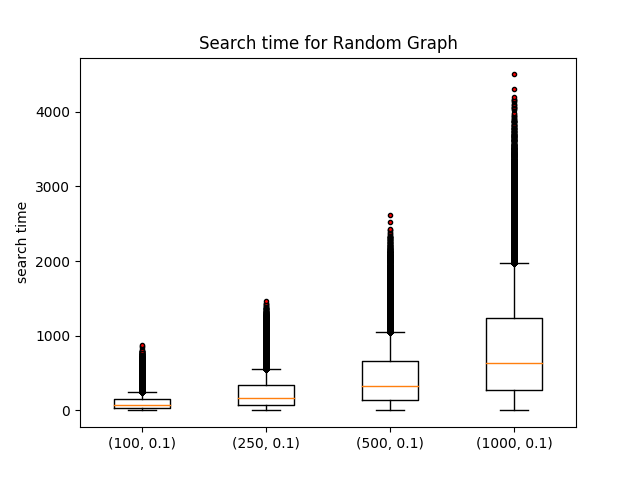
\includegraphics[width=1\textwidth]{{box/box-random_graph-n-search_time_v2-avg}.png}
        \subcaption{iterate until the vertex's number of neighbours}
        \label{rg:n2}
    \end{minipage} \hfill
    \caption{Search Time Distribution for Random Graph when only n changes}
    \label{rg:n}
\end{figure}
\noindent
Figure-\ref{rg:n1} and figure-\ref{rg:n2} had a constant probability p and an increasing n. As n increased the search time increased which was an expected outcome as more edges and vertices would be iterated over. The performance of the algorithm described in the previous section was the one used in figure-\ref{rg:n1}, it did not significantly improved the search time (the difference if there is any is barely noticable from the box plots in both figures \ref{rg:n1} and \ref{rg:n2}). The median search time across all graph instances was slightly more than half of n and the shape of the graph persisted as well.
\begin{figure}[H]
    \centering
    \begin{minipage}{0.48\textwidth}
        \centering
        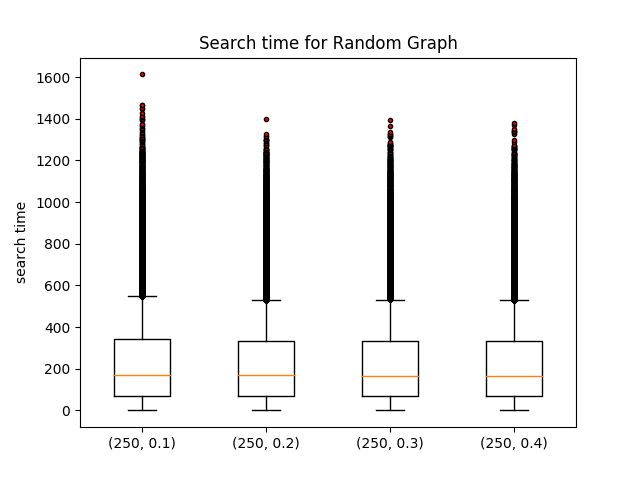
\includegraphics[width=1\textwidth]{{box/box-random_graph-p-search_time_v1-avg}.png}
        \subcaption{Only iterate until average number of neighbours}
        \label{rg:p1}
    \end{minipage}\hfill
    \begin{minipage}{0.48\textwidth}
        \centering
        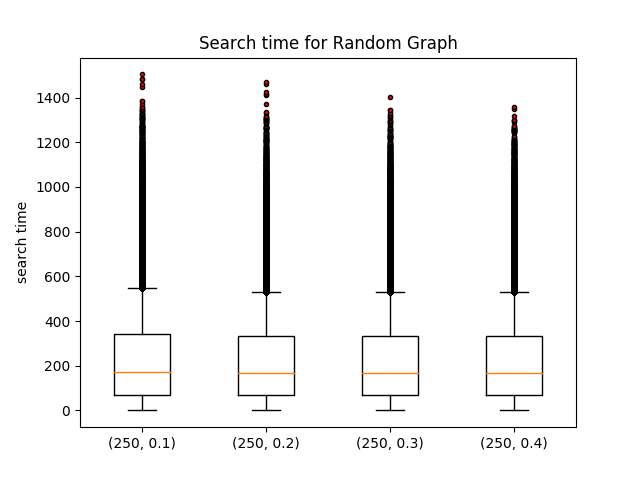
\includegraphics[width=1\textwidth]{{box/box-random_graph-p-search_time_v2-avg}.png}
        \subcaption{iterate until the vertex's number of neighbours}
        \label{rg:p2}
    \end{minipage} \hfill
    \caption{Search Time Distribution for Random Graph when only n changes}
    \label{rg:p}
\end{figure}
\noindent
Figure-\ref{rg:p1} and figure-\ref{rg:p2} had a constant n and an increasing p. As p increased the search time decreased but only very slightly. \\

\noindent
Based on the search algorithm, the search time increased as n increased however it slightly decreased as p increased in a random graph. The shape of the distribution remains skewed to the right with a lot of outlier values throughout all the distributions in figures \ref{rg:n} and \ref{rg:p}.

\subsection*{Search Ring Group Graph}
\subsubsection*{Search Algorithm}
By definition all vertices in a Ring Group graph are part of a group, and adjacent groups have higher probability (p) of having an edge between their vertices than with other groups which have a lower probability (q). So, the most basic strategy for searching this graph is by moving to the closest group or if possible to a group adjacent to the target vertex and look for the target in that group because of the higher probability. Unlike Random graph not all vertices are connected with the same probability and the group number is part of the vertex id so it helps narrow the search significantly. Based on this, the search in a Ring Group graph was implemented as follows:
\begin{itemize}
    \item Inputs:
    \begin{itemize}
        \item The graph
        \item The graph parameters - (m, k, p, q)
        \item The start vertex id - (numerical id, group)
        \item The target vertex id - (numerical id, group)
    \end{itemize}
    \item Initialize a variable for search time and set it to 0
    \item Create a variable for the probability to move to a vertex that is closer to the target's group than the current vertex and set it to be equal to p; call it prob\_close. 
    \item check if p is greater than 0.5, if it is then set p to 1 - p
    \item start an infinite loop until the target vertex is found:
    \begin{itemize}
        \item shuffle the current vertex's neighbours list (at the beginning it is the start vertex)
        \item Iterate over the neighbours list:
        \begin{itemize}
            \item increment the search time by 1 for every iteration that happens
            \item if the neighbour's id matches the target's id then stop, break out of the loop and return the search time
            \item else if the neighbour's group is the same as the traget's group then move to that neighbour with a probability p (the probability for vertices in adjacent groups to have an edge), otherwise keep track of this neighbour in adjacent\_neighbour variable 
            \item else if the neighbour's group is closer to the target than the current vertex's move to that neighbour with the probability that we set at the beginning of this algorithm (prob\_close) otherwise keep track of this neighbour - closest\_not\_adjacent\_v - the same way as the previous condition
            \item else move to this neighbour with a probability of q (probability of an edge )
        \end{itemize}
        \item if no moves has been made check if adjacent\_neighbour has been assigned and move to it, otherwise check if closest\_not\_adjacent\_v has been assigned and move to it. If neither values are assigned move to the last queried neighbour
    \end{itemize}
\end{itemize}
The assigned value for prob\_close was determined through trial and error and proved to provide the best results (figure-\ref{rggs:521v1} and figure-\ref{rggs:521v2}). The condition for when p is more than 0.5 is similar to the one in the random graph, making it less likely to move to another vertex in the group to find the target vertex as the high probability indicates that it is very likely that the target vertex is connected to the current vertex. For adjacent\_neighbour and closest\_not\_adjacent\_v variables, only one neighbour is stored at a time so if another neighbour with the same condition is encountered that neighbour will be stored instead and as the neighbours list is shuffled with every move it is less likely this neighbour will be the same if the current vertex is returned to at some point.

\subsubsection*{Search Time Distribution}
To insure that the graph instance was connected, networkx package was used for both creating the graph using networkx graph structure and then checking if it's connected (all nodes have an edge between them). The following plots are the search time against the number of instances that achieve that time evaluated for 30,000 randomly picked pairs of vertices normalized and averaged over 10 instances of the ring group graph and averaged again:
\begin{figure}[H]
    \centering
    \begin{minipage}{0.48\textwidth}
        \centering
        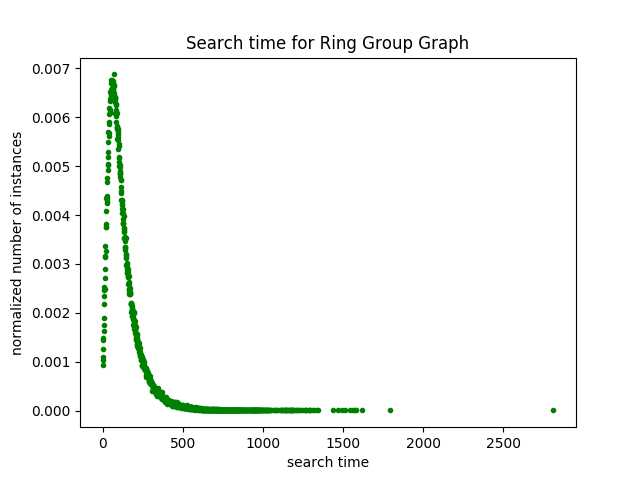
\includegraphics[width=1\textwidth]{{search-time/ring_group_graph-50-20-0.45-0.01-search_time_v2-avg}.png}
        \subcaption{Search time distribution normalized}
        \label{rgg:nd}
    \end{minipage}\hfill
    \begin{minipage}{0.48\textwidth}
        \centering
        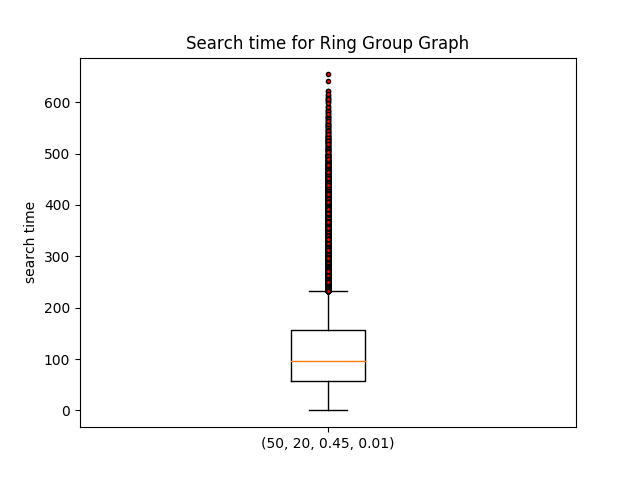
\includegraphics[width=1\textwidth]{{box/box-ring_group_graph-50-20-0.45-0.01-search_time_v2-avg}.png}
        \subcaption{Box-plpot respresentation of the search time distribution}
        \label{rgg:bx}
    \end{minipage} \hfill
    \caption{Search Time Distribution for Ring Group Graph when m = 50, k = 20, p = 0.45 and q = 0.01}
    \label{rgg:n}
\end{figure}
\noindent
Figure-\ref{rgg:nd} is an example of a search distribution for a ring group graph when the graph parameters are m = 50, k = 20, p = 0.45 and q = 0.01. Similarly to the search distribution for random graph, the box-plot will be used to represent the distribution as it is much simpler to interupt like figure-\ref{rgg:bx}; some of the outlier values might not be included, those outliers have a low number of occurance so they were discarded in the box-plot and only the main distribution was included. In this case, the distrbution was slightly skewed to the right with a lot of outlier values. The shape of the distribution was more defined than the distribution for random graph and the median was closer to the middle of the inter-quartile range in the box-plot \ref{rgg:bx}. There were more nodes in this graph to search than the random graph and still the range of the search time values was much lower than the random graph searches. Around $50\%$ of the instances had a search time that was around 100 and majority of the instances had a search time less than 300. \\

\noindent
Before invesitigating the effect of paramater changes to the search in a ring group graph, the following plot demonstrates the benefit of introducing the variable prod\_close to the algorithm:
\begin{figure}[H]
    \centering
    \begin{minipage}{0.48\textwidth}
        \centering
        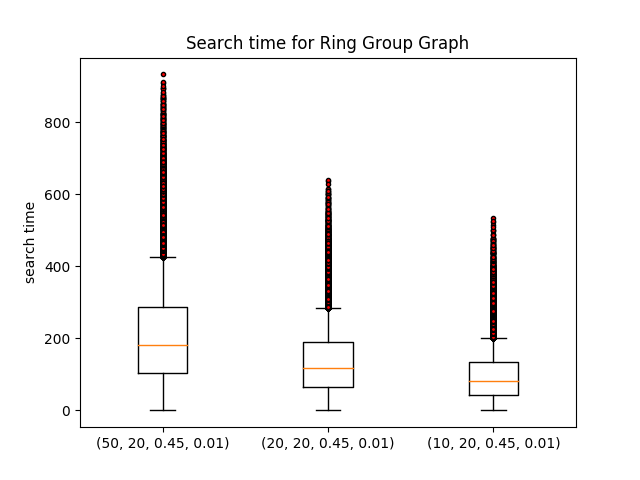
\includegraphics[width=1\textwidth]{{box/box-ring_group_graph-50-20-10-search_time_v1-avg}.png}
        \subcaption{without the probability to move to a closer neighbour}
        \label{rggs:521v1}
    \end{minipage}\hfill
    \begin{minipage}{0.48\textwidth}
        \centering
        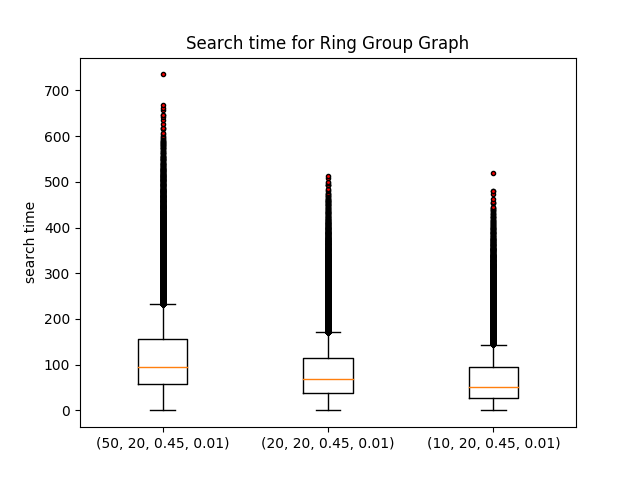
\includegraphics[width=1\textwidth]{{box/box-ring_group_graph-50-20-10-search_time_v2-avg}.png}
        \subcaption{with the probability to move to a closer neighbour set to p}
        \label{rggs:521v2}
    \end{minipage} \hfill
    \caption{Ring Group Graph parameters: p = 0.45, p = 0.01, k = 20 and m is decreasing}
    \label{rggs:521}
\end{figure}
As shown in figure-\ref{rggs:521v2}, the search time for the ring group graph with the specified paramaters was much lower with prob\_close introduced and set to the value of probability p. Even as the value of m was decreasing the search time was still lower in figure-\ref{rggs:521v2} than figure-\ref{rggs:521v1}. The outlier values were less as well. This proves by making it more likely for the target to move closer to its adjacent group allows for faster search time (dependent on the value of p).\\ 

\noindent
The remaining plots will look into the search time values as the paramater for the ring group graph:
\begin{figure}[H]
    \centering
    \begin{minipage}{0.48\textwidth}
        \centering
        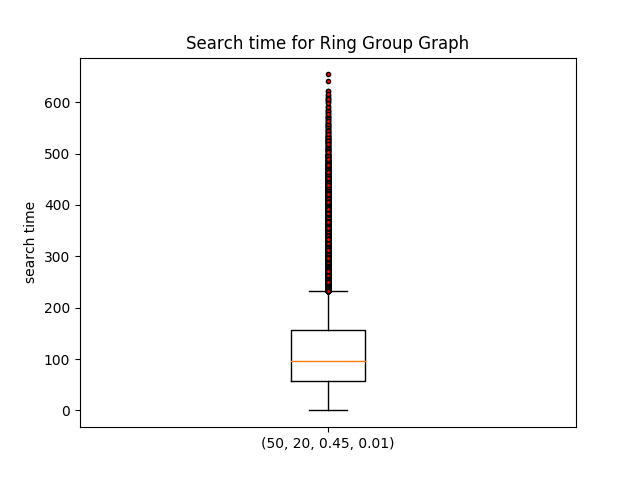
\includegraphics[width=1\textwidth]{{box/box-ring_group_graph-50-20-0.45-0.01-search_time_v2-avg}.png}
        \subcaption{Search Time distribution when m is greater than k}
        \label{rggs:q5245}
    \end{minipage}\hfill
    \begin{minipage}{0.48\textwidth}
        \centering
        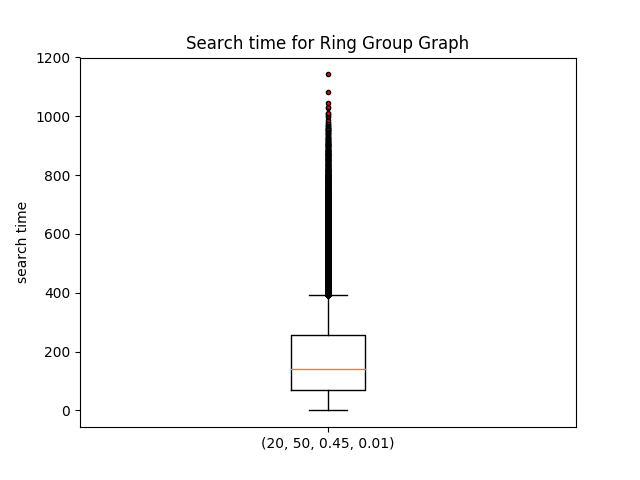
\includegraphics[width=1\textwidth]{{box/box-ring_group_graph-20-50-0.45-0.01-search_time_v2-avg}.png}
        \subcaption{Search Time distribution when k is greater than m}
        \label{rggs:q2545}
    \end{minipage} \hfill
    \caption{Ring Group Graph parameters: p = 0.45, q = 0.01}
    \label{rggs:q01}
\end{figure}
\noindent
In this figure, the total number of the nodes is equal and the same p and q values are applied to m and k. As shown in figure-\ref{rggs:q5245}, the search time was much lower when m was greater than k. The shape of the distribution however was almost identical. Compared to figure-\ref{rggs:q5245}, the search time in figure-\ref{rggs:q2545} was almost twice as much; majority of instances had a search time less than 250 in \ref{rggs:q5245}, in contrast in \ref{rggs:q2545}, around 50\% of instances had a search time between 150 and 400. \\

\begin{figure}[H]
    \centering
    \begin{minipage}{0.48\textwidth}
        \centering
        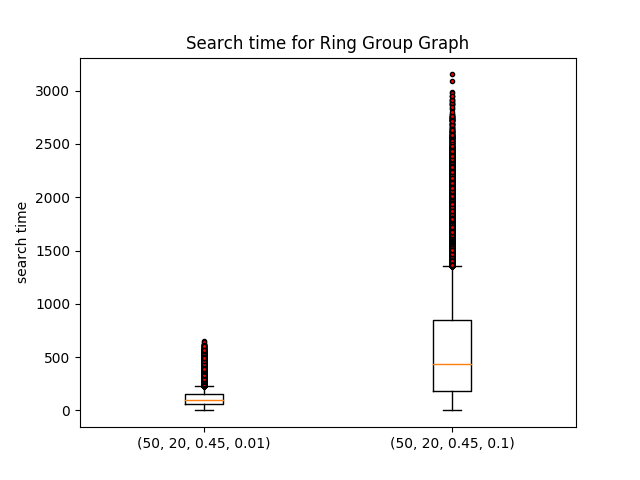
\includegraphics[width=1\textwidth]{{box/box-ring_group_graph-50-20-search_time_v2-avg}.png}
        \subcaption{Search Time distribution when m is greater than k and q is changing}
        \label{rggs:q52}
    \end{minipage}\hfill
    \begin{minipage}{0.48\textwidth}
        \centering
        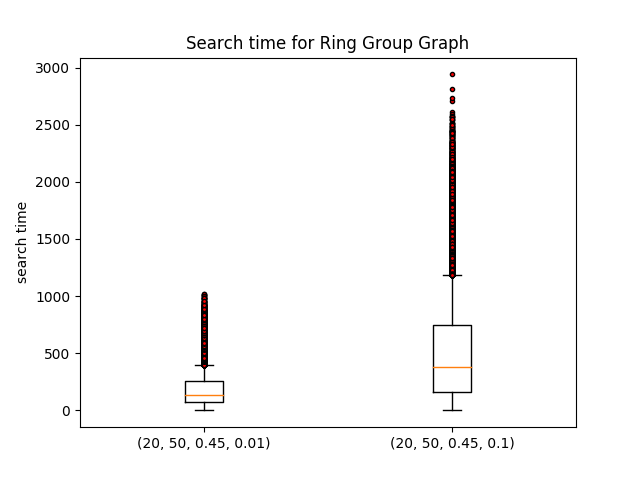
\includegraphics[width=1\textwidth]{{box/box-ring_group_graph-20-50-search_time_v2-avg}.png}
        \subcaption{Search Time distribution when k is greater than m and q is changing}
        \label{rggs:q25}
    \end{minipage} \hfill
    \caption{Ring Group Graph parameters: p = 0.45}
    \label{rggs:q}
\end{figure}
\noindent
This figure extends the comparison made in figure-\ref{rggs:q01}. The value of q was increased to 0.1, this resulted in the search time for both pairs of m and k in \ref{rggs:p25} and \ref{rggs:p52} to significantly increase (more random edges has been introduced) The distribution is also more skewed to the right and the box-plot is similar to the plot for a random graph; the upper quartile covers way more search time values than the lower quartile and the median is slightly further down from the center of the box. 

\begin{figure}[H]
    \centering
    \begin{minipage}{0.48\textwidth}
        \centering
        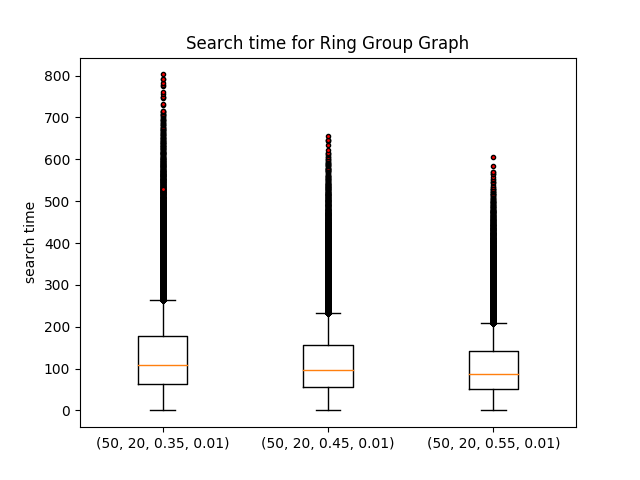
\includegraphics[width=1\textwidth]{{box/box-ring_group_graph-50-20-p-search_time_v2-avg}.png}
        \subcaption{Search Time Distribution when m is greater than k and changing p}
        \label{rggs:p52}
    \end{minipage}\hfill
    \begin{minipage}{0.48\textwidth}
        \centering
        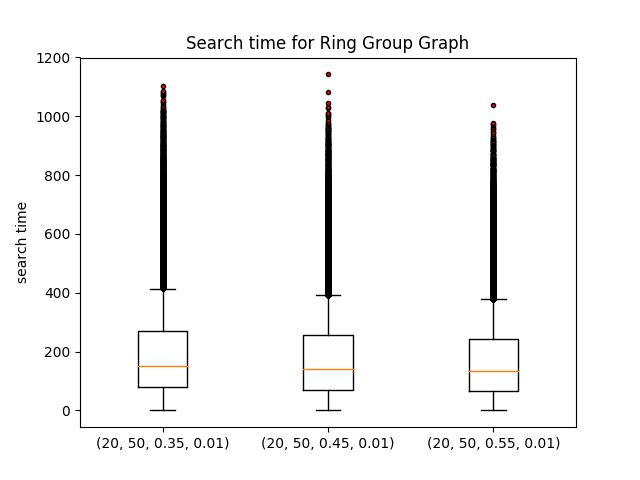
\includegraphics[width=1\textwidth]{{box/box-ring_group_graph-20-50-p-search_time_v2-avg}.png}
        \subcaption{Search Time Distribution when k is greater than m and changing p}
        \label{rggs:p25}
    \end{minipage} \hfill
    \caption{Ring Group Graph parameters: q = 0.01}
    \label{rggs:p}
\end{figure}
\noindent
On the other hand, when p increaseed and q remained constant, the search time generally decreased as shown in figure-\ref{rggs:p}. The decrease was more noticable when m was greater than k, figure-\ref{rggs:p52}. This indicates that the search algorithm implemented for the ring group graph much favours high p values, low q values and m to be greater than k. This doesn't mean that this algorithm is less effective for the other cases but it is more optimized for the previous conditions. 

\begin{figure}[H]
    \centering
    \begin{minipage}{0.48\textwidth}
        \centering
        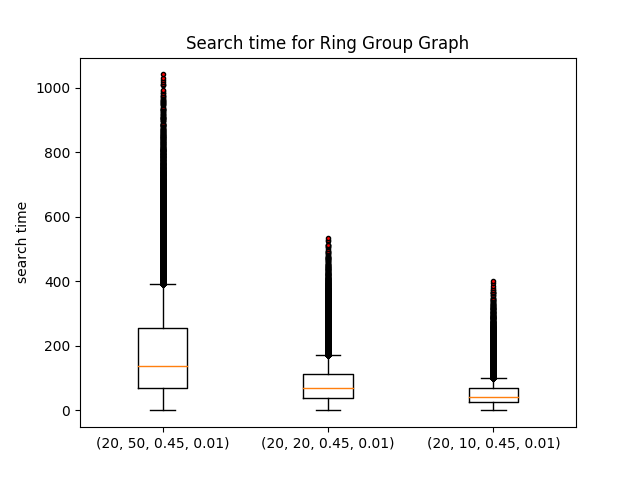
\includegraphics[width=1\textwidth]{{box/box-ring_group_graph-10-20-50-search_time_v2-avg}.png}
        \subcaption{Search Time Distribution with changing k and m = 20}
        \label{rggs:125v2}
    \end{minipage}\hfill
    \begin{minipage}{0.48\textwidth}
        \centering
        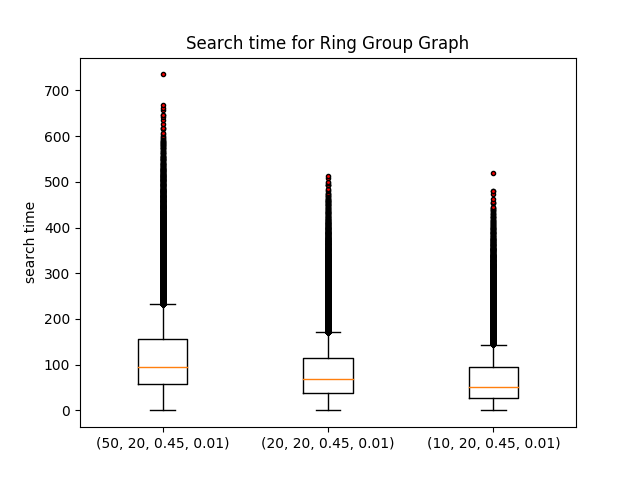
\includegraphics[width=1\textwidth]{{box/box-ring_group_graph-50-20-10-search_time_v2-avg}.png}
        \subcaption{Search Time Distribution with changing m and k = 20}
        \label{rggs:521v22}
    \end{minipage} \hfill
    \caption{Ring Group Graph parameters: p = 0.45, q = 0.01}
    \label{rggs:125}
\end{figure}
Figure-\ref{rggs:125} further looks into the changes in the distribution; the value of k decreased as m, p and q remained constant, figure-\ref{rggs:125v2}, and the value of m decreased as k, p and q remained constant, figure-\ref{rggs:521v22}

\begin{figure}[H]
    \centering
    \begin{minipage}{0.48\textwidth}
        \centering
        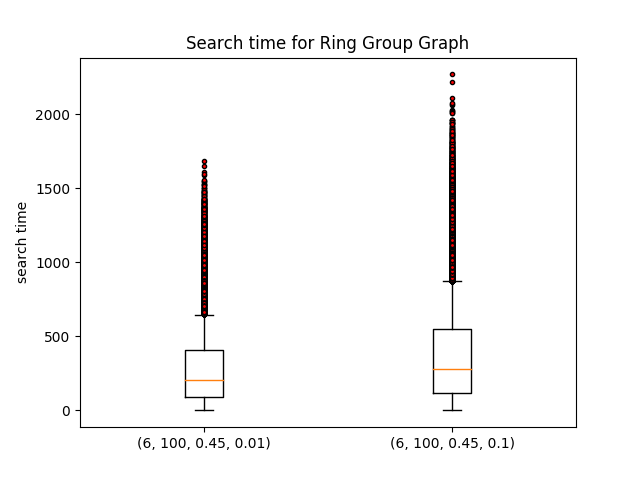
\includegraphics[width=1\textwidth]{{box/box-ring_group_graph-6-100-search_time_v2-avg}.png}
        \subcaption{Search Time Distribution with changing q}
        \label{rggs:s61}
    \end{minipage}\hfill
    \begin{minipage}{0.48\textwidth}
        \centering
        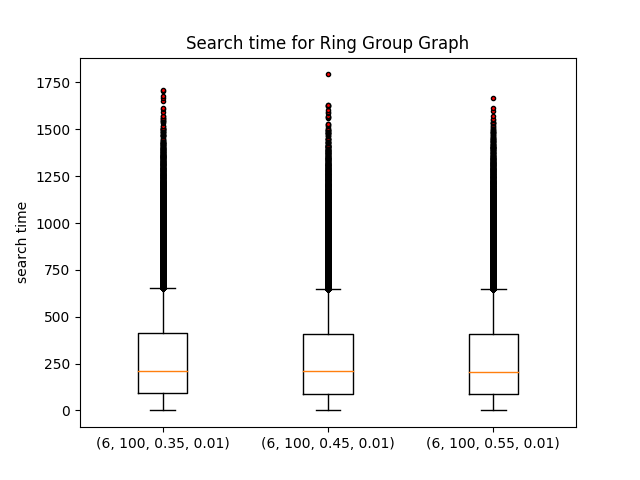
\includegraphics[width=1\textwidth]{{box/box-ring_group_graph-6-100-p-search_time_v2-avg}.png}
        \subcaption{Search Time Distribution with changing p}
        \label{rggs:sp}
    \end{minipage} \hfill
    \caption{Ring Group Graph parameters: m = 6, k = 100}
    \label{rggs:s}
\end{figure}
\noindent
The paramaters picked for the ring group graph instances tested here were based on the results in Figure-\ref{rggs:mgp} and Figure-\ref{rggs:kgp}. The figures demonstrate the effictiveness of the algorithm by looking into relationship between the search time and the probability p (groups are more connected) tested over low q probabilities (less chance of shortcuts appearing the graph). The algorithm performs better with greater m values and greater p values.

\end{document}